% Instructions to change to html version:
% Comment out:
%  minipage, multicols,columnbreak, mathbf, hrule
% Replace \\] with \[ and \) with \(
% Enclose graphics in figure environments and add captions
% Re-tag \df environments as sections, subsections, etc.
% Command Line Code to Create html version:
%First: pdflatex -shell-escape filename.tex                                   
%Second, for each figure: inkscape "filename-figure1.pdf" -o "filename-figure1.png"
% Third: htlatex filename.tex "ht5mjlatex.cfg, charset=utf-8" " -cunihtf -utf8"

\documentclass[10pt]{article}

%\usepackage{tikz, pgf,pgfplots,wasysym,array}
%\usepackage{wasysym,array}

\usepackage{amsmath,amssymb}

\ifdefined\HCode
  \def\pgfsysdriver{pgfsys-tex4ht-updated.def}
\fi 
%\ifdefined\HCode
%  \def\pgfsysdriver{pgfsys-dvisvgm4ht.def}
%\fi 
\usepackage{tikz}
\usetikzlibrary{calc,decorations.markings,arrows}
\usepackage{pgfplots}

\pgfplotsset{compat=1.12}
\usepackage{myexternalize}
\usetikzlibrary{calc,decorations.markings,arrows}
\usepackage{framed}
\usepackage[none]{hyphenat}

\input{../../../common/1336_header_test.tex}
% % !tex root = ./exam_2.tex
\usepackage[nomessages]{fp}% 
\usepackage{rotating}
\usepackage{graphicx}
\usepackage{sectsty}
\usepackage{xparse}
\usepackage{tikz}
\usepackage{pgf,pgfplots}
	% For the histogram ?
	\pgfdeclarelayer{background}% determine background layer
	\pgfsetlayers{main,background}% order of layers

\usepackage{tkz-berge}
\usetikzlibrary{calc,graphs,arrows,backgrounds,decorations.pathreplacing}
%Not found:\usetikzlibrary{graphs.standard,quotes}
\usetikzlibrary{shapes}
		\tikzset{
		  dot hidden/.style={},
		  line hidden/.style={},
		  dot colour/.style={dot hidden/.append style={color=#1}},
		  dot colour/.default=black,
		  line colour/.style={line hidden/.append style={color=#1}},
		  line colour/.default=black
		}
\NewDocumentCommand{\rot}{O{45} O{1em} m}{\makebox[#2][l]{\rotatebox{#1}{#3}}}%



\begin{document}



\newcommand{\an}{\lbrace a_n \rbrace}
\newcommand{\Sum}{\sum_{n=1}^\infty }
\newcommand{\Sumzero}{\sum_{n=0}^\infty }

\everymath{\displaystyle}

\renewcommand{\myTitle}{\	MATH 1336: Calculus III}

\renewcommand{\mySubTitle}{Section 8.5, Part 1: Intro to Power Series}% \vspace*{-.25in}}
%~\hfill Name: \underline{~~~~~~~~~~~~~~~~~~~~~~~~~~~~~~~~~~~~~~~~~~~~~~~}

\lectTitle{\vspace*{-.5in}\myTitle}{\vspace*{.1in}\mySubTitle \vspace*{-.2in}}




\hspace*{-.8in}%\begin{minipage}{1.25\textwidth}

\setlength{\columnseprule}{.4pt}
\setlength{\columnsep}{3em}
\section*{Power Series Definition:}
A series of the form:
\[
\Sumzero c_n (x-a)^n = c_0 + c_1 (x-a) + c_2 (x-a)^2 + c_3 (x-a)^3 +\ldots
\]
is called a \textbf{Power Series centered at \(x=a\)}.\\
 (Power Series in \((x-a)\), Power Series about \(a\))\\
 
\underline{\textbf{Notes:}}
\begin{itemize}
\item A Power Series \textbf{always} converges at the center: \(x=a\).
\item Adopt the convention that \(0^0 = 1\).
\item By definition: \(0! = 1\).
\end{itemize}
 %%\end{multicols}%\( \\~\\~\\
 
% \vspace*{.25in}
 %\columnbreak
 
\subsection*{Power Series Convergence Theorem:}
For a given Power Series, \(\Sumzero c_n (x-a)^n\), there are three possibilities:
 \begin{enumerate}[(i)] 
 \item The series converges \textit{only} when \(x=a\). 
 \item The series converges for all \(x\).
 \item There is some \(R>0\) such that the series converges if \(|x-a|<R\) and diverges if \(|x-a|>R\).
 \end{enumerate}
 
 %\end{multicols}
 
 %\hrule
 \vspace*{.1in}
 
\subsection*{Radius \& Interval of Convergence:}
%\begin{multicols}{2}


 \(R\) is the \textbf{radius of convergence}, as described above.\\
 The \textbf{interval of convergence}, \(I\), is the interval of all the \(x-\)values where the series converges.
 % \vspace*{.25in}
 
 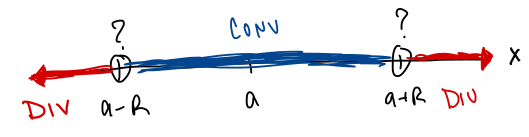
\includegraphics[width=.75\textwidth]{Ch8s5-Power-Series-Interval.png}
 
 %\columnbreak
 
 \underline{\textbf{Strategy:}}\\
 \begin{enumerate}
 \item Use the Ratio Test (or Root Test) to find the radius of convergence.
 \item If you need to know the convergence behavior at the endpoints of the interval of convergence, use another series test!
 \end{enumerate}

%\end{multicols}
\vspace*{.2in}

%\end{framed}

%\end{minipage}

%\vfill

\section*{Examples we will work through together:}
%Find the radius and interval of convergence for the following series:

\begin{enumerate}[{Example }1:]

\item Motivation: For which values of \(x\) does the following series converge?\\
 \( \qquad \Sumzero \frac{x^n}{n^2}\)
 
 \vfill
 
 \pagebreak

%\addtocounter{enumi}{1}

\hspace*{-.75in Find the radius and interval of convergence for the following series:}
\item \( \qquad \Sumzero n!\ x^n\)
\vfill

%\pagebreak

\item \( \qquad \Sum \frac{x^{2n}}{(2n)!}\)
\vfill

\item \( \qquad \Sum \frac{(x-1)^n}{n}\)
\vfill


%
%\item The \(p-\)Power Series: \(\qquad \Sum	\frac{x^n}{n^p}\)
\vfill
%
%\item \(\Sumzero \frac{n(x+5)^n}{4^{n+1}}\)
%\vfill
\end{enumerate}

\pagebreak

\section*{Problems for Group Work}

\begin{enumerate}
\item Find the radius and interval of convergence for the following power series:

\(\qquad \Sumzero \frac{n(x+5)^n}{4^{n+1}}\)
\vfill

%%\begin{multicols}{2}
%\begin{enumerate}
%
%\item \(\Sumzero \frac{(-5)^n (x-10)^n}{n!}\)
%
%\vspace*{.75in}
%
%\item \(\Sumzero e^n(x-2)^n\)
%
%\vspace*{.75in}
%
%\item \(\Sum \frac{(-2)^n x^n}{n^2}\)
%
%\vspace*{.75in}
%
%\item \(\Sumzero x^n\)
%
%\vspace*{.75in}
%
%\end{enumerate}
%%\end{multicols}
\vfill

\item \textbf{Strategy Practice:}\\
For each of the following series, state which test you would use to determine the convergence or divergence behavior, and explain why.

(You do not have to carry out the test in detail, but follow the argument long enough to make sure your reasoning would work.)

\begin{enumerate}
%\begin{multicols}{2}

\item \(\Sum \frac{n}{2n+1}\)\vspace*{.75in}

\item \(\Sum \frac{(-2)^n}{\sqrt{n}}\)\vspace*{.75in}

\item \(\Sum \frac{1}{\sqrt{n^3-n^2}}\)\vspace*{.75in}

\item \(\sum_{k=1}^\infty \frac{2^k k!}{(k+2)!}\)\vspace*{.75in}
%\end{multicols}

\vfill

\end{enumerate}


\end{enumerate}
\end{document}
